\problemname{Dome Construction}

The world's largest indoor water park is built inside a hemispherical dome that
was once used as an aircraft hangar. The park attracts more than $10\,000$
visitors per day and is big enough that it even has its own tropical
micro-climate with clouds forming inside.

Management would like to expand business operations by opening another branch
in the dome of your local cathedral. The micro-climate is a key selling point,
so to really capitalise on the cathedral they asked you to expand the dome's
radius so that it contains at least a given number of clouds. A cloud is
contained if its centre is on or inside the boundary of the dome.

% \begin{figure}[h!]
%   \centering
%   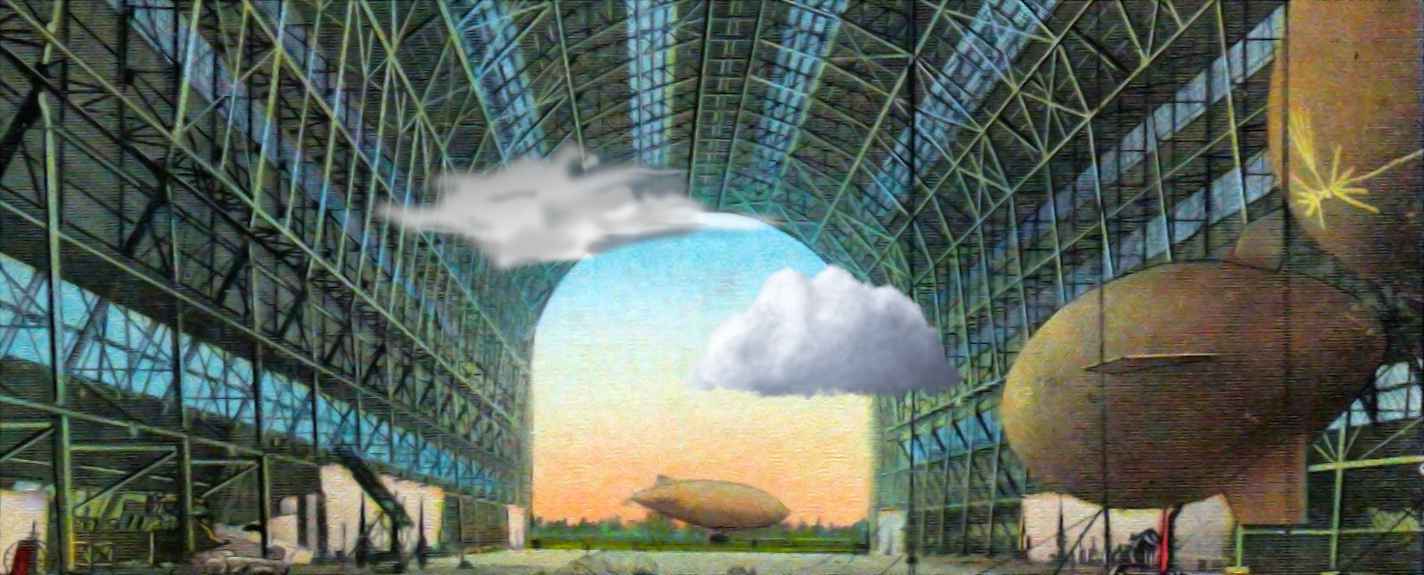
\includegraphics[width=1.0\textwidth]{hangar}
%  \label{fig:dome}
% \end{figure}

You are a cloud engineer by trade, and hence a competent meteorologist. You
already identified several potential clouds close by and plotted them in three
dimensions relative to the centre of the current structure. In order to capture
enough of them, how large do you need to make the radius of the dome?

\section*{Input}

\begin{itemize}
  \item The first line contains the number of clouds you found, $n$, and the
        number that must be contained, $k$, respectively
        ($1 \le k \le n \le 10^5$).
  \item The next $n$ lines each contain three real numbers $x_i, y_i, z_i$, the
        coordinates of the $i$th cloud relative to the centre of the dome
        ($0 \le |x_i|, |y_i|, |z_i| \le 10^6$). Every cloud has a non-negative
        $y$-coordinate.
\end{itemize}

\section*{Output}

Output the minimum radius of the dome required to enclose at least $k$ points.
Your answer must be accurate to an absolute or relative error of $10^{-6}$.
